\documentclass{article}

\usepackage[german]{babel}
\usepackage[a4paper,top=2cm,bottom=2cm,left=3cm,right=3cm,marginparwidth=1.75cm]{geometry}
\usepackage{amsmath}
\usepackage{graphicx}
\usepackage[colorlinks=true, allcolors=blue]{hyperref}
\usepackage{algorithmic}
\usepackage{algorithm}
\usepackage[font=small,labelfont=bf]{caption} % Required for specifying captions to tables and figures
\usepackage{booktabs}
\usepackage{siunitx}
\bibliographystyle{plain}


\begin{document}
\begin{titlepage}
      \begin{center}
          \Huge
          \text{Universit\"at Innsbruck} \\
          \vspace{1cm} % Add some vertical space
          \Large
          Institut f\"ur Informatik \\
          \vspace{1cm}
          
\includegraphics[width=7cm]{universitaet-innsbruck-logo-cmyk-farbe.jpg}

          \Huge
          \textbf{Heuristische Optimierung der Operatorplatzierung in verteilten Stream-Verarbeitungssystemen} \\
          \vspace{3cm} % Add more vertical space

          \Large
          Cedric Immanuel Sillaber \\
          Matrikel-Nr: 12211124
          
          \vspace{1cm}
          \large
          VU Einführung ins Wissenschaftliche Arbeiten \\
          \vspace{4cm}
          \normalsize
          Betreuer:\\ Prof. Dipl.-Ing. Dr. Thomas Fahringer
          
          \vfill 
          
          \large
          \today
      \end{center}
  \end{titlepage}
\begin{abstract}
In den vergangenen Jahren wurden Big Data Applikationen stets populärer. 
Da die Anzahl der Daten umfangreicher wird, werden effiziente Ansätze für 
verteilte Stream-Datenverarbeitung (SVS) benötigt.
Das Problem der Operatorplatzierung ist ein entscheidender Performancefaktor. 
Für das Lösen dieses Problems gibt es jedoch keine 
effiziente Lösung. Diese Arbeit beschäftigt sich mit einer effizienten heuristischen Methode, die versucht,
die optimale Lösung zu approximieren. 
\end{abstract}

\section{Einführung}
Im Zuge der fortschreitenden Digitalisierung entwickelte sich Datenverarbeitung zu einem zentralen Aspekt der Modernität.
Der Erfolg vieler Konzerne beruht auf der Expertise, wie kontinuierliche Datenmengen effizient verarbeitet werden.
Rund um die Uhr werden Daten gesammelt, die in Echtzeit verarbeitet werden müssen. 
SVSs wie (zitat nötig) sammeln, filtern und verarbeiten Daten. Die Daten werden von einer großen Menge an 
Geräten produziert. Derartige Systeme werden beispielsweise in der Analyse von Finanzmärkten \cite{k5}, 
Verabreitung von Sozialen Netzwerk-Interaktionen und der Beobachtung von Network-Traffic \cite{k5} 
eingesetzt. Ein SVS besteht aus einer Menge von unabhängigen Operatoren, die eine spezifische
Funktionalität ausführen. Aus der Unabhängigkeit der Operatoren lässt sich die Möglichkeit folgern, 
dass die Rechner im Netzwerk (Cloud-Edge \cite{k6}) lokalisiert sind, anstatt in der Cloud.
In solch einem System stehen zahlreiche Ressourcen zur Verfügung. 
Als Operatorplatzierung bezeichnet man das Problem, 
die Operatoren im System optimal auf verfügbare Knoten zu platzieren.
In Abbildung 1 ist ein verteiltes SVS abgebildet. Eine Anzahl von Datenquellen P produziert Daten, die zu den Senken C führen. Die Operatoren 
werden in der Abbildung als SBON bezeichnet. Das Operatorplatzierungproblem (OPP) beschäftigt sich mit der Frage, 
welche physichen Knoten die Operatoren hosten sollen \cite{network-aware-op}. 

Für die Evaluation solcher Modelle werden diverse Quality-of-Service Attribute herangezogen. 
Dazu gehören Durchsatz, End-zu-End Latenz und Verfügbarkeit \cite{efficient-operator-placement} \cite{cardellini-optimal_operatorplc}.  Der Ansatz in dieser Arbeit versucht sich auf generalisierte QoS Attribute 
zu fokusieren, die einfach angepasst werden können \cite{efficient-operator-placement}.
Diese Arbeit fokusiert sich auf einen Ansatz, der bekannte Heurisiken kombiniert und optimale Lösungen effizient approximiert. Der Ansatz bezieht sich auf keine spezifische
Implementierung und ist somit modell-frei. Somit kann diese Lösung für verschiedene Systeme angewendet werden.

Die optimale systematische Position in solch einem System stellt einen maßgeblichen Performancefaktor dar. 
Die Lösung dieses Problems ist jedoch NP-hard \cite{cardellini-optimal_operatorplc}.

\begin{center}
    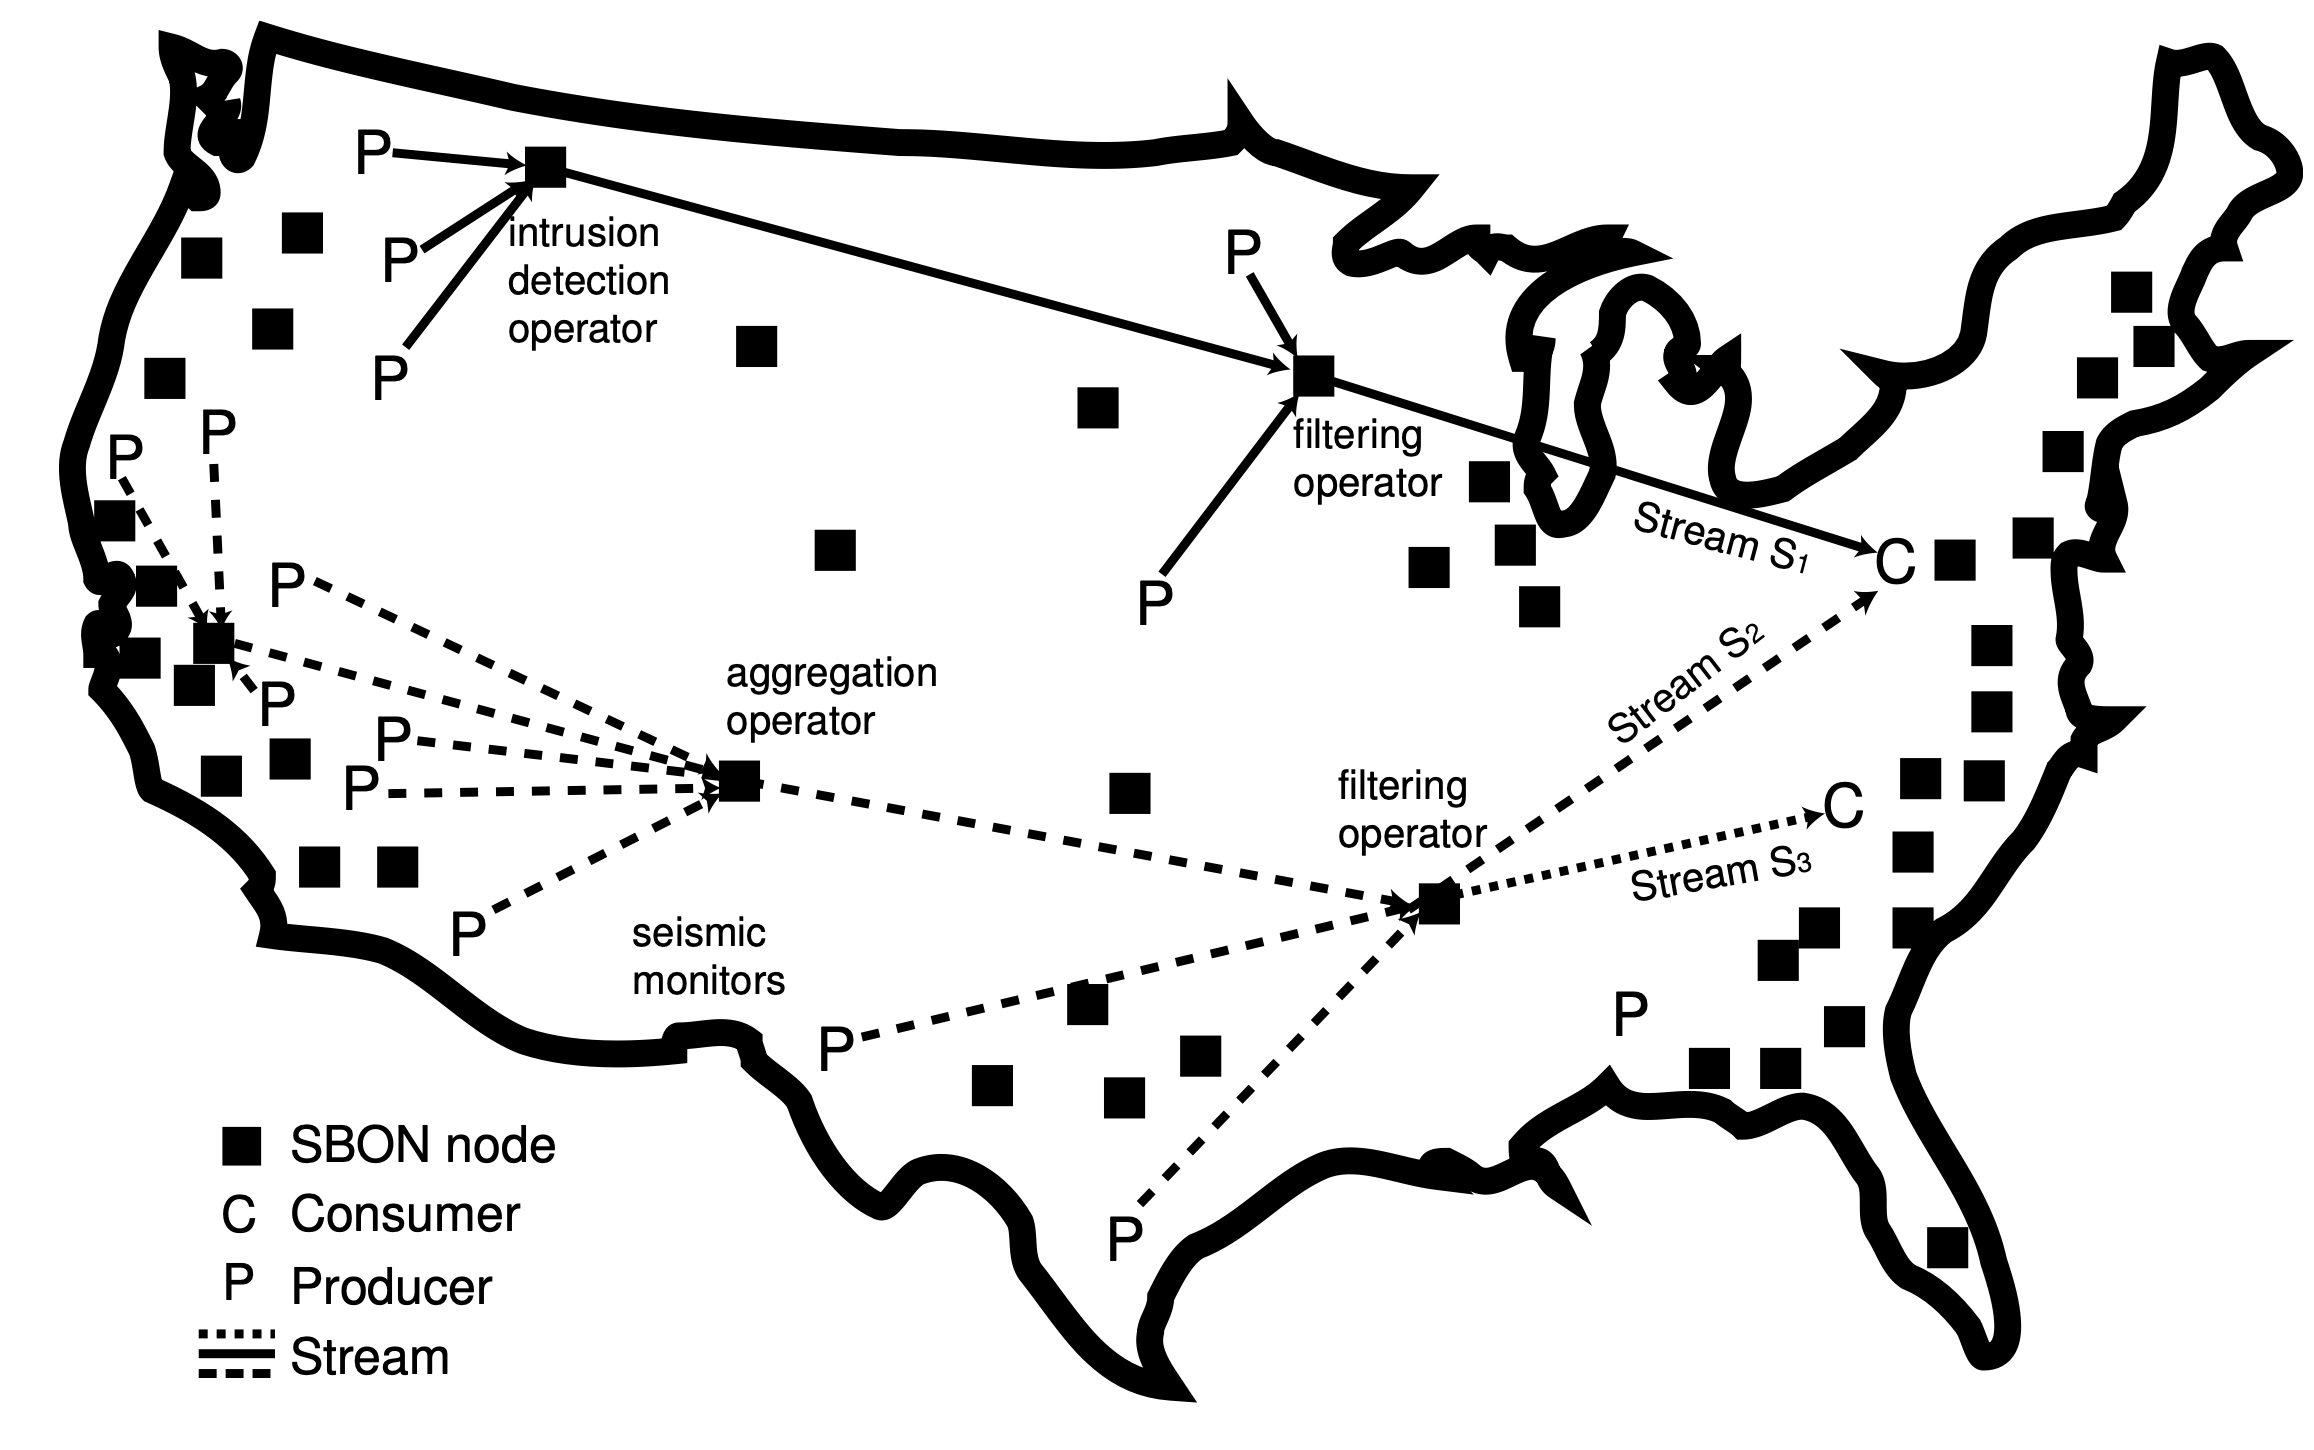
\includegraphics[width=0.5\linewidth]{SVS.png}
    \captionof{figure}{Stream Verarbeitungssystem, Quelle: \cite{network-aware-op}.} 
\end{center}



\section{Definitionen}
Um eine konkrete Optimierung des Problems beschreiben zu können, ist es notwending die Problematik formal zu formulieren. 
Im folgenden Kapitel %oder section??
wird eine formale Abstraktion des Operatorplatzierungproblems vorgestellt. Zuerst wird das Datenstrom- 
und das Ressourcenmodell \ref{SVS-Definition} defininiert. Beide Modelle werden mittels Graphentheorie formuliert und beschreiben 
ein SVS. 
Folglich wird das Problem der Operatorplatzierung mithilfe der zuvor definierten Modelle formuliert \ref{OPP-Definition}. 


\subsection{Definition von verteilten Streamdatenverarbeitungssystemen}  \label{SVS-Definition}  % evt "formale definition ..."
%In diesem Abschnitt werden die Grundlagen verteilter Stream-Verarbeitungssysteme eingegangen. Wir geben eine formale Darstellung SVSs und geben eine Definition für das Operatorplatzierungs Problem. Zu 
SVSs basieren auf einer Menge an verteilten Computer Ressourcen, die zusammen ein komplexes System ergeben. 
Dieser Sachverhalt kann mittels Graphentheorie beschrieben werden. Grundsätzlich gibt es zwei Abstraktionen solcher Systeme. 
Erstens das Datenstrom Modell und zweitens das Ressourcen Modell. 
Beide Systeme werden mit gerichteten, gewichteten zykelfreien Graphen $G = (V,E)$ dargestellt. 

\textit{Datenstrom Modelle} werden durch $G_{svs} = (V_{svs}, E_{svs})$ beschrieben. In diesem Modell beschreiben Knoten $u \in V_{svs}$ Operatoren im System. 
Zusätzlich sind in $V_{svs}$ Datenquellen und Datenbecken enthalten. Man spricht hierbei von Datenbecken (vgl. "sink"), ein Punkt, an dem die Berechnungen der Operatoren zusammekommen. 
Zu den Operatoren gehören auch sogenannte \textit{pinned} Operatoren \cite{efficient-operator-placement}, 
die Datenquellen und -becken beinhalten. Kanten $(u,v) \in E_{svs}$ beschreiben Datenstreams 
zwischen den Operatoren $u$ und $v$.  Ein Stream ist ein kontinuierliche Sequenz von Daten. 

\textit{Ressourcen Modelle} werden durch den Graphen $G_{res} = (V_{res}, E_{res})$ dargestellt. 
Dabei wird der logische Zusammenschluss zwischen verfügbaren Computing Ressourcen beschrieben. Der Knoten $u \in V_{res}$ 
repräsentiert solch eine Ressource. In diesem Modell beschreiben Kanten $(u,v) \in E_{res}$ 
eine logische Verknüpfung zwischen dem Rechnerressourcen $u$ und $v$.
% vielleicht Fig. 1 aus efficient operator placement hinzufügen?.


\subsubsection{Angepinnte Operatoren}



\subsection{Definition von Operatorplatzierungproblem} \label{OPP-Definition}
Ein Operator kann aus politischen, sicherheitsbezüglichen oder topologichen Gründen \cite{cardellini-optimal_operatorplc} nicht auf jedem Knoten 
$i \in V_{svs}$ im Datenstrommodell platziert werden. 
Für jeden Operator $i \in V_{svs}$ gibt es eine Menge an Kandidatressourcen $V_{res}^i$ (Schreibweise wie in \cite{efficient-operator-placement}).

Das Operator Problem bezeichnet eine Abbildung zwischen den genannten Modellen. Die Abbildung wird eingeschränkt,
damit die zu minimierenden QuS Attribute eingeschränkt werden. Folglich wird der optimale Kandidat $u$ in den Kandidatenressourcen $V_{res}^i$
gesucht, damit Operator $i$ auf Knoten $u$ platziert wird.
Hierbei bezieht sich das Problem auf die Inkonsistenz zwischen 
logisch benachbarten Operatoren im Ressourcen Modell $G_{res}$ und optimalen Entscheidungen der Operatoren im Datenstrom Modell $G_{svs}$.

Um das Problem formal zu definieren, verwenden wir den binären Ausdruck $x_{i,u}$ $i \in V_{svs}, u \in V_{res}: x_{i,u} = 1$ wenn Operator $i$
auf dem Rechner $u$ platziert wird, andernfalls $x_{i,u} = 0$

\[ 
    \begin{gathered}
        \operatorname*{arg\,min}_\theta F(x) \\
        \sum_{i \in V_{svs}} C_i x_{i,u} < C_u \quad \forall u \in V_{res} \\ % constrain: node resource
        \sum_{u \in V_{res}^i} x_{i,u} = 1 \quad \forall i \in V_{dsp} \\ % constrain: node only placed on candidate resources
        x_{i,u} \in \{0,1\} \quad \forall i \in V_{svs}, u \in V_{res}^i
    \end{gathered}
\] 

Hierbei wird die Funktion $F(x)$ bezüglich ausgewählten QoS minimiert. Dieses multi-objective Optimierungsproblem wird durch 
Simple Additive Weight technique \cite{yoon-multiple-optimization} zu einem single-objective Problem umgewandelt.
Für typische QoS Attribute wie Antwortzeit, Verfügbarkeit und Netzwerkverwendung \cite{efficient-operator-placement} wird die Funktion $F(x)$ wie folgt defininiert:
\[ 
    \begin{gathered}
        F(x) = w_r \frac{R(x) - R_{min}}{R_{max} - R_{min}} 
        + w_a \frac{log A_{max} - log A(x)}{log A_{max} - log A_{min}} 
        + w_z \frac{Z(x) - Z_{min}}{Z_max - Z_min} 
    \end{gathered}  \label{to-miminize-function}
\] 
wo $R(x)$, $A(x)$ und $Z(x)$ die QoS Attribute und $w_r, w_a, w_z \geq 0$ Gewichtungen sind. $R_{min}$, $R_{max}$, $A_{min}$, $A_{max}$, $Z_{min}$ und $Z_{max}$ sind die minimalen und maximalen Werte der QoS Attribute.
$w_r + w_a + w_z = 1$


%QoS: pplication response time Rx, the application availability A(x), and the network usage Z(x).


Mithilfe einer \textbf{penalty function} werden die  Verbindungen zwischen zwei spezifischen Knoten bezüglich der QoS Attribute bewertet. Dadruch wird ein Vergleich 
der Rechnerressourcen möglich. Dabei werden die Links zwischen $u \in V_{res}^i$ möglich. Auf die penalty function wird im folgenden eingegangen.




\section{Heuristiken} \label{Heurisiken}
% erwähnen dass es sich um ein model free characteristic handelt
Wie in \cite{cardellini-optimal_operatorplc} gezeigt, ist das 
Operatorplatzierungproblem NP-hard.
Da die initiale Platzierung der Operatoren eine tragender Faktor
in der Performance einnimmt, werden effiziente Heuristiken benötigt. 
In dieser Abreit wird eine effiziente Methode vorgestellt, die 
zu einer approximierten Optimalösung führt. 
Dieser Ansatz beinhaltet eine Kombination mehrere bekannter Heuristiken, die die Funktion $F$ aus \ref{to-miminize-function} minimieren.  
Ein Greedy First-Fit Ansatz in Kombination mit einer lokalen Suche findet meist lokale Optima. 
Um dem entgegenzuwirken wird dieser Ansatz mit einer Tabu Search verbunden. 
Somit werden häufiger \cite{efficient-operator-placement} globale Optima gefunden. 

Ein Greedy First-Fit Algorithmus wird für das Bin-packing Packing Problem verwenden, 
aber auch oft für das Operator Placement Problem \cite{k7}\cite{k8}.
Da diese Heuristik meist nur lokale Optima findet, werden andere Ansätze hinzugezogen. 
Zum einen wird Local-Search verwendet, ein Verfahren, 
das mit einem Greedy Ansatz über einen Teil der Funktion iteriert. Da auch dieses
Verfahren dazu neigt, lokale Optima auszuwählen, wird zusätzlich Tabu Search implementiert. 
Die drei Heuristiken werden gekonnt kombiniert und führen somit zu einer besseren Approximation. 

\subsection{Penalty Function} 
% penalty function ist für Links, nicht für knoten!
Die Auswahl von verschiedenen Möglichkeiten $u \in V_{res}^i$ bringt Einbussen mit sich. Diverse Ressourcen haben verschiedene Lokalitäten,
deren Performance durch Netzwerkdynamiken beeinflusst wird. Da die Daten übertragen werden müssen, kommen nicht vorhersehbare Network Delays dazu. Hierzu müssen Network Delay, 
Bandbreite und Netzwerkgeschwindigkeit\cite{efficient-operator-placement} betrachtet werden.


\subsection{Greedy First Fit} \label{greedy-first-fit}
Diese Heuristik wird  für das Bin-Packing Problem verwendet, um eine optimale Lösung anzunähern \cite{greedy-first-fit}. 
Für jeden Operator werden die verfügbaren Ressourcen $v \in V_{res}$ in einer Liste sortiert. Die Sortierung basiert auf der summierte penalty function $\delta$
zwischen $v$ und den angepinnten Operatore $P$. Folglich:

\[ 
    \begin{gathered}
        u_i \in P \text{, wobei P = angepinnten Operatoren} \\
        \sum_{i=0}^{|P|} \delta(v, u)
    \end{gathered} 
\] 

Ausgewählt wird der erste Rechner in der Liste, der den Operator aufnehmen kann. 
Mittels Breitensuche werden für alle Operatoren Plazierungen bestimmt. Die daraus resultierenden Operatorplatzierungen werden als eine Konfiguration bezeichnet. 
Diese Heuristik 

%greedy frist fit no delta beschreiben



\subsection{Local Search} \label{local-search}
Die lokale Suche ist eine iterative Heuristik zur Optimierung von Lösungen in der Nachbarschaft einer Ausgangskonfiguration.
Dabei iteriert diese Methode über die Konfiguration, die aus der Greedy First Fit Heuristik resultieret. Der Algorithmus dafür wird im Algorithmus 1 \ref{local-search-algo} gezeigt. 
Dieser Algorithmus durchläuft drei Schritte: Zunächst wird eine initiale Konfiguration durch den Greedy First Fit berechnet.
 Anschließend wird eine Nachbarschaft von ähnlichen Konfigurationen bestimmt, und schließlich wird die beste Lösung in dieser Nachbarschaft gefunden. 
 Um die Nachbarschaft zu bestimmen, wird zunächst eine sortierte Liste $L$ erstellt, basierend auf der penalty function $\delta$ wie in \ref{greedy-first-fit}.
Mit dieser Liste wird dann eine initiale Konfiguration $S$ durch den Greedy First Fit Algorithmus erstellt (Zeile 6). \\



Solange bessere Platzierungen der Operatoren gefunden werden, iteriert die lokale Suche über die Konfigurationen  (Zeile (insert)). 
Eine Verbesserung wird durch einen niedrigeren Wert der Zielfunktion $F$ definiert. 
Die Suche nach besseren Konfigurationen basiert auf den drei Funktionalitäten \textit{co-locate operators, swap resources, Bewegen von Operator}. \\


\begin{algorithm}[H]
    \caption{Local Search}
    \begin{algorithmic}[1]
        \STATE \textbf{function} $\mathrm{localSearch}(G_{dsp}, G_{res})$
        \STATE \textbf{Input}: $G_{\text{dsp}}$, DSP application graph
        \STATE \textbf{Input}: $G_{\text{res}}$, computing resource graph
        \STATE $P \leftarrow$ resources hosting the pinned operators of $G_{\text{dsp}}$
        \STATE $L \leftarrow$ resources of $G_{\text{res}}$, 
        sorted by the cumulative link penalty with respect to nodes in $P$
        \STATE link penalty with respect to nodes in $P$
        \STATE $S \leftarrow$  solve GreedyFirstFit($G_{\text{dsp}}$, $L$)
        \STATE \textbf{do}

        \STATE \hspace{\algorithmicindent} $F \leftarrow$  value of the objective function for $S$
        \STATE \hspace{\algorithmicindent} $S \leftarrow$  improve $S$ by colocating operators
        \STATE \hspace{\algorithmicindent} $S \leftarrow$  improve $S$ by swapping resources
        \STATE \hspace{\algorithmicindent} $S \leftarrow$  improve $S$ by relocating a single operator
        \STATE \hspace{\algorithmicindent} $F' \leftarrow$ value of the objective function for S

        \STATE \textbf{while} $F'  < F$ \textbf{do}
        \STATE \hspace{\algorithmicindent} \textbf{return} $S$
        \STATE \textbf{end function}
    \end{algorithmic}
\end{algorithm}


Zwei Operatoren $i,j \in G_{svs}$, wobei $i$ auf $u \in G_{res}$ und $j$ auf $v \in G_{res}$ platziert ist, werden als \textit{co-located} bezeichnet, 
wenn $i$ und $j$ zusammen auf einem Rechner platziert sind. Somit befindet sich $i$ und $j$ auf entweder $u$ oder $v$.\\
Bei \textit{swap resources} wird der Operator $i$, der auf $u \in G_{res}$ platziert ist, auf eine neue Ressource $v \in G_{res}$ aus $L$ verschoben. 
Für den Fall, dass zuerst $n$ Operatoren $j_1, j_2, ..., j_n$auf $u$ alloziert sind, werden diese auf $v$ verschoben. \\ 
Die Funktionalität \textit{move single locator}  bewegt nur einen einzelnen Operator $i$ von $u \in G_{res}$ zu $v \in G_{res}$, wobei $v$ aus $L$ ausgewählt wird. 


% \vspace{0.7cm}
Das Zusammenführen von Operatoren auf eine gemeinsame Rechnerressource ermöglicht es, 
verwandte Aufgaben in eine bessere Lokalität zu platzieren, was QoS verbessern kann. 
Das Austauschen von Operatoren strebt eine Eliminierung/Minimierung von ressourcelichen Engpässen an. 
Durch das Bewegen einzelner Operatoren werden somit auch lokale Engpässe minimiert.
Dafür werden die Konfigurationen so angepasst, dass  Datenströme gleichmäßig verteilt werden.   \\
Sobald keine Verbesserungen mehr gefunden werden, terminiert die lokale Suche und gibt die beste Konfiguration zurück. 
Dabei ist es wichtig zu beachten, dass wie \ref{greedy-first-fit} nur eine Approximation ist und in einer lokal-optimalen Lösung enden kann. 

 


\subsection{Tabu Search}
Die Heurisitische lokale Suche ist abhängig von der initialen Konfiguration und terminiert nur bedingt mit einer globalen optimalen Lösung für das Operatorplatzierungproblem. 
Um dem entgegenzuwirken, wird die Heurisik zur \textit{Tabu Suche} \cite{glover-tabu-search} erweitert.  In dieser Methode wird über mehrere Anfangskonfigurationen iteriert, 
die anhand der Lokalen Suche nicht unmittelbar zu einer Verbesserung führen. Durch diese Eweiterung
werden Lösungen evaluiert, die bei einer lokalen Suche nicht betrachtet werden. \\
Der Algortihmus kann in die folgenden Schritte unterteilt werden \cite{glover-tabu-search-tutorial}. Zuerst wird eine Ausgangslösung berechnet.
Anhand dieser Ausgangslösung wird eine Nachbarschaft bestimmt. Die Nachbarschaft wird um die sogenannten Tabu Züge verkleinert. 
Aus der resultierenden Nachbarschaft wird die beste Lösung bestimmt und ausgewählt. Am ende der iteration wird die Tabuliste basierend auf einem Tabukriterium aktualisiert.


\begin{algorithm}[H]
    \caption{Tabu Search}
    \begin{algorithmic}[1]
        \STATE \textbf{function} $\mathrm{tabuSearch}(G_{dsp}, G_{res})$
        \STATE \textbf{Input}: $G_{\text{dsp}}$, DSP application graph
        \STATE \textbf{Input}: $G_{\text{res}}$, computing resource graph

        \STATE $S^* \leftarrow$ undefiniert
        \STATE $F^* \leftarrow \infty$
        \STATE $S' \leftarrow \text{localSearch}(G_{dsp}, G_{res})$   //local optimum
        \STATE $F' \leftarrow$ objective function value for $S'$
        \STATE $S  \leftarrow S'$
        \STATE $tabuList \leftarrow$ create new tabu list and append $S$
        \STATE \textbf{do}

        \STATE \hspace{\algorithmicindent} improvement $\leftarrow false$
        \STATE \hspace{\algorithmicindent} $S \leftarrow$  local search for $S$, excluding solutions in $tabuList$
        \STATE \hspace{\algorithmicindent} \textbf{if} $F = F^*$ \textbf{and} $S \notin tabuList$ \textbf{then} $tabuList$.append($S$) 
        \STATE \hspace{\algorithmicindent} \textbf{end if}

        \STATE \hspace{\algorithmicindent} \textbf{if} $F < F^*$ \textbf{and} $S \notin tabuList$ \textbf{then} 
        \STATE \hspace{\algorithmicindent} \hspace{\algorithmicindent} $S^* \leftarrow S; F^* \leftarrow F$
        \STATE \hspace{\algorithmicindent} \hspace{\algorithmicindent} $tabuList$.append($S$)
        \STATE \hspace{\algorithmicindent} \hspace{\algorithmicindent} improvement $\leftarrow true$

        \STATE \hspace{\algorithmicindent} \textbf{end if}
        \STATE \hspace{\algorithmicindent} limit $tabuList$ to the latest $tabuList_{max}$ placement configurations
        \STATE \textbf{while} improvement
        \STATE \textbf{if} $F' < F^*$ \textbf{then} $S^* \leftarrow S'$ \textbf{end if}
        \STATE \textbf{return} $S^*$

    \end{algorithmic}
\end{algorithm}


Der Algorithmus startet mit einer Ausgangskonfiguration $S'$, die von der Greedy-First-Fit-Heuristik erstellt wurde (Zeile 6). \\ \\
Von Zeile 10 bis 21 durchläuft er eine Schleife, die in jeder Iteration nach einer besseren Lösung $S$ in der Nachbarschaft sucht. 
Diese Suche wird mittels lokaler Suche durchgeführt. Dabei werden Lösungen aus $S$ ausgeschlossen, die in der Tabuliste enthalten sind (Zeile 12). \\ \\
Die Tabuliste $tabuList$ ist anfangs leer und beinhaltet nach der ersten Iteration die letzten $tabuList_{max}$ Platzierungen. 
Dadurch wird verhindert, dass die Schleife unendlich iteriert.
In jeder iteration wird die neue Lösung $S$ mit der Zielfuntion $F$ evaluiert (Zeile 13). %penalty function
Wenn die jetzige Lösung $S$ besser als die vorherige Lösung $S^*$ ist, wird $S$ als die beste Lösung $S^*$ gespeichert (Zeile 15, 16). \\ \\

Sobald die Schleife terminiert ist, wird die neue beste Lösung $S^*$ mit der Ausgangslösung $S'$ verglichen. Die insgesamt beste Lösung wird zurückgegeben. 



%\vspace{0.7cm}

Mit dieser Heuristik wird der Lösungsraum nach besseren Approximationen des Optimums durchsucht. 
Im Vergleich zur Greedy First Fit \ref{greedy-first-fit} und der 
lokalen Suche \ref{local-search} bietet die Tabu-Suche eine erweiterte Fähigkeit zur Exploration 
des Lösungsraums und kann somit zu verbesserten Lösungen führen.



% vgl greedy, greedy no delta, local search, tabu search tabelle aus paper
\section{Evaluation}
Die oben angeführten Heuristiken \ref{Heurisiken} werden in einem Experiment aus \cite{efficient-operator-placement} evaluiert. 
Für das Expermiment werden die drei Heuristiken Greedy First Fit, Greedy First Fit ohne penalty function und die lokale Suche verglichen. 
Als bezugsnorm wird die optimale Lösung des Operatorplatzierungsproblems verwendet. Im Experiment von \cite{efficient-operator-placement} werden mehrere Heuristiken
bewertet, die hier der Einfachheit halber nicht aufgeführt werden. Auch die genauen Details der Hardware sind nicht relevant für die Evaluation. 


\subsection{Infrastruktur}
Für die Untersuchung werden drei verschiedene Netzwerktopologien herangezogen. 
Diese Topologien beschreiben die verteilten Infrastrukturen der SVS. 
Diesbezüglich werden die Rechnerressourcen und deren Verbindungen definiert, sowie die inter-knoten latenz \cite{efficient-operator-placement}.
Die drei untersuchten Topologien sind in Abbildung \ref{topologies} dargestellt. Dabei werden simple sequentielle, replicated und Diamaond Topologien verwendet.\\

\noindent
\begin{minipage}{0.45\textwidth}
    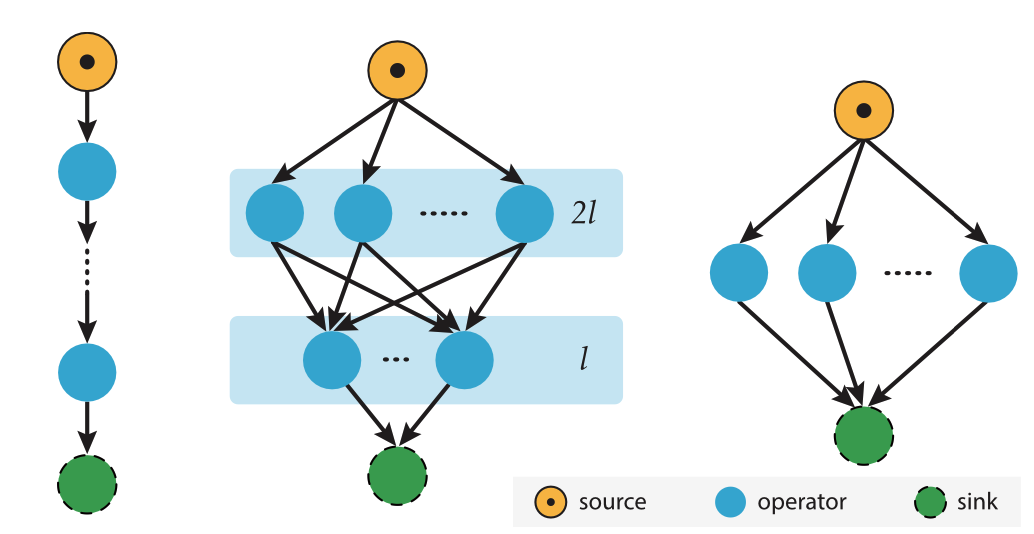
\includegraphics[width=0.75\linewidth]{topologies.png}
\captionof{figure}{Sequentielle, replizierte und Diamant-Topologie, Quelle: \cite{efficient-operator-placement}. }
\label{topologies}
\end{minipage}
\hspace{10pt}
\begin{minipage}{0.5\textwidth}
    In den dargestellten Topologien hat jede Schicht mindestens einen Operator. 
    Die erste und letzte Schicht verfügen jeweils über einen Operator, die Quelle und das Becken. 
    Alle Ressourcentopologien haben die gleiche Anzahl an Ressourcen.
\end{minipage}



\subsection{Experimentelle Ergebnisse}

Für das Experiment werden die Laufzeit (LZ) und die Qualitätseinbuße (QE) betrachtet \cite{efficient-operator-placement}.
Diese Merkmale werden mit der optimalen Lösung verglichen. Rt beschreibt die benötigte Zeit, 
um eine Lösung zu finden, pd beschreibt die Abweichung von der optimalen Lösung. 
Zusätzlich wird der Beschleunigungsfaktor (bf) definiert als $bf = rt_{optimal} / rt_i$, wobei $rt_i$ die Zeit für die Heuristik $i$ ist.
Le wird definiert als $le_i = \frac{F_i - F_{ODP}}{1 - F_{ODP}}$ \cite{efficient-operator-placement}, 
wobei $F_i$ die Zielfunktion der Heuristik $i$ ist.

Wie in \ref{OPP-Definition} definiert, werden im Experiment Verfügbarkeit, 
Netzwerklatenz und Antwortzeit als QoS selektiert und folglich mit der Straffunktion minimiert. 


% ODP definieren


\subsubsection{Generelle Ergenisse}

Die Berechnung der Optimalösung weist eine effiziente Laufzeit für Diamandtopologien basierte auf. 
Diese Berechnung ist in unter einer Sekunde verfügbar. Bei replizierten und sequentiellen Topolgien benötigt die Berechnung deutlich länger. 
Für replizierte Topologien dauert die Evaluation mehr als 8 Stunden (=32193 aus Tabelle). \\
\begin{table}[htbp]  
    \centering
    \caption{Evaluation der Heuristiken}
    \begin{tabular}{llllll}
    \toprule
    Policy                           &       & DA        & SA              & RA                & Overall Average Value                  \\
    \midrule
    ODP                              &LZ 36s &  0.1      & 41.4             & 915.2            &                  \\
                                     &LZ 100s&  0.8      & 2174.8           & 32193.9          &                  \\
    \cmidrule{1-5}
    Lokale Suche                     &BF     &  0.68     & 150.54           & 353.07           & 215.81           \\
                                     &QE     &0\%        & 1\%              &4\%               & 1\%              \\
    Tabu Suche                       &BF     &  0.31     & 65.91            & 64.93            & 83.53            \\
                                     &QE     &0\%        & 1\%              &4\%               & 1\%              \\           
    Greedy First Fit                 &BF     &  454.40   & $56 \cdot 10^4$  & $12 \cdot 10^6$  & $11 \cdot 10^6$  \\
                                     &QE     &0\%        & 7\%              &5\%               &11\%              \\
    Greedy First Fit (keine $\delta$)&BF     &  454.40   & $56 \cdot 10^4$  & $12 \cdot 10^6$  & $11 \cdot 10^6$  \\
                                     &QE     &34\%       & 7\%              &24\%              & 19\%             \\
    \bottomrule
    \multicolumn{4}{l}{\footnotesize Tabelle aus des Experiments \cite{efficient-operator-placement}, BF = Beschleunigungsfaktor,}\\
    \multicolumn{4}{l}{\footnotesize QE = Leistungseinbuße, LZ = Laufzeit}\\
    \end{tabular}
\end{table} \label{experiment-tabelle}


Die Berechnung der Optimalösung weist eine effiziente Laufzeit für Diamandtopologien basierte auf. 
Diese Berechnung ist in unter einer Sekunde verfügbar. Bei replizierten und sequentiellen Topolgien benötigt die Berechnung deutlich länger. 
Für replizierte Topologien dauert die Evaluation mehr als 8 Stunden (=32193 aus Tabelle).

Aus Tabelle \ref{experiment-tabelle} ist zu erkennen, dass Greedy First Fit die schnellste Lösung bietet. 
Da die übrigen Heuristiken auf Greedy First Fit basieren, entspricht das auch den Erwartungen. 
Trotz des hohen Beschleunigungsfaktors $bf$ liefern Greedy First Fit und Greedy First Fit (ohne $\delta$) degradierte Lösungen. 
Somit ergibt sich ein Kompromiss zwischen der Qualität der Lösung und der Laufzeit des Algorithmus. 
Auffällig ist die Diskrepanz zwischen der Greedy First Fit Implementierung mit und ohne Straffunktion $\delta$. 
Bei Beschleunigungsfaktoren ähnlicher Größenordnung resultieren die verschiedenen Implementierungen 
in unterschiedlichen Lösungsqualitäten, besonders bei Diamant- und replizierten Topologien.

Lokale Suche ist im Experiment schneller als Tabu Suche, jedoch ist die Qualität der Lösung geringer. 
Somit bietet die Tabu Suche die beste Operatorplatzierung, mit der längsten Laufzeit. 
Trotzdem stellt sich die Berechnung als viel effizienter heraus als die optimale Lösung. 
Während die Laufzeit der optimalen Lösung für replizierte Topologien mehr als 8 Stunden beträgt, benötigt die Tabu Suche 8,2 Minuten. 
Lokale Suche findet in x Minuten eine Lösung. Dabei beträgt die Qualitätseinbuße bei beiden Methoden 1\%. 
In der Degradation der Performance ist bei Lokalen Suche und Tabu Suche kein klarer Unterschied zu erkennen. 

Es gibt in diesem Experiment keinen Gewinner. Zwischen den Heuristiken gibt es Kompromisse zwischen Schnelligkeit und Genauigkeit. 

\section{Konklusion und Ausblick}
In dieser Arbeit wurden mehrere Heuristiken vorgestellt, die das NP-schwere Problem der Operatorplatzierung approximieren. 
Dabei handelt es sich um bekannte Methoden, die auch für andere NP-schwere Probleme utilisiert werden. Mittels einer Straffunktion
werden die Heuristiken auf QoS Attribute optimiert. \\
Die vorgestellten Heuristiken basieren auf Greedy First Fit und erweitern dessen Funktionalität (Lokale Suche und Tabu Suche).
Die Heuristiken wurden in einem Experiment für drei verschiedene SVS Architekturen evaluiert. 
Bei der Evaluation wurde auf die Laufzeit und die Qualität der Lösung eingegangen. 
Daraus resultierte, dass keine der Heuristiken eine klare Überlegenheit aufweist. 
Beispielsweise führte die Greedy First Fit Heuristik zu einer schnellen Lösung, die aber qualitativ degradiert war.
Die Lokale Suche und die Tabu Suche berechneten bessere Platzierungen, erforderten jedoch mehr Zeit.
Dennoch weisen die Heuristiken eine deutliche Steigerung der Laufzeit gegenüber der optimalen Lösung auf. 
\\

In Zukunft werden wir noch komplexere Heuristiken entwerfen, die das OPP Problem noch besser approximieren. 
Die vorgestellten Methoden werden zur Kompilierzeit verwendet, was bei dynamischen Veränderungen nicht effizient ist. 
Deswegen wollen wir uns auf Laufzeit adaptivfähige Heuristiken fokusieren. 
Zudem wollen wir die erneute Konfiguration während der Laufzeit analysieren, damit Big Data Anwendungen auf verändernde Bedingungen reagieren können. 



\newpage
\bibliography{biblio}

\end{document}